%--------Apendice
%--------Emir Muñoz Jiménez
%--------13-10-2010

\chapter{Manual de Usuario}
\label{cap:manual}

En este anexo se encuentran las instrucciones de uso del software desarrollado, lo requerimientos mínimo y los pasos necesario para su instalación.

\section{Requerimientos}

Los requerimientos mínimos necesarios para la instalación y funcionamiento del software son.

\begin{itemize}
\item C++11 (g++ 4.8+)
\item OpenCV 2.4.9
\item Boost 1.54
\item SO linux
\item 4GB RAM
\item Procesador intel COREi3 1.9GHz
\item Espacio libre en disco superior a 5GB
\end{itemize}

Los requerimientos recomendados para un correcto funcionamiento son.

\begin{itemize}
\item C++11 (g++ 4.8+)
\item OpenCV 2.4.9
\item Boost 1.54
\item Linux mint 17 / Ubuntu 14.04
\item 8GB RAM
\item Procesador intel COREi5 2.6Ghz
\item Espacio libre en disco superior a 20GB
\end{itemize}


\section{Instalaci\'on}

Para la instalación hay que copiar el contenido de la carpeta sscaThesis en el directorio donde se desea instalar y ejecutar el comando \textit{make}.

Para el funcionamiento es necesario crear los archivos de lista con el path de las imágenes a utilizar la estructura para los archivos de lista es la siguiente donde la lista superior contiene las otras.

\begin{itemize}
\item Lista según uso (Entrenamiento positivo, Entrenamiento negativo, Pruebas).
\subitem * Lista según tamaño de ventana.
\subsubitem     - Lista de los path de las imágenes.
\end{itemize}


\section{Utilización}

Para la ayuda en el programa utilizar el comando

\begin{lstlisting}
./main.o --help 
\end{lstlisting}

Para para realizar detección y normalización ejecutar el siguiente comando

\begin{lstlisting}
./main.o -p <Archivo lista ejemplos positivos> -n <Archivo lista ejemplos negativos> -t <Archivo lista ejemplos de prueba>  -c <Seleccion del clasificador, soportados svm & boost>
\end{lstlisting}

Para realizar la evaluación de sensibilidad espacial utilizar el si

\begin{lstlisting}
sh evaluate.sh <directorio con las matrices *.mat> <nombre del archivo de salida>
\end{lstlisting}


\section{Entradas y Salidas}


A continuación se expone ejemplos de las entradas y salidas del programa.

\subsection{Entradas}

El archivo de entrada de imágenes positivas contiene una lista con las direcciones de cada imagen.

\begin{lstlisting}
INRIAPerson/train_crop_32x64/pos/crop_000010.png
INRIAPerson/train_crop_32x64/pos/crop_000011.png
INRIAPerson/train_crop_32x64/pos/crop_000603.png
INRIAPerson/train_crop_32x64/pos/crop_000606.png
INRIAPerson/train_crop_32x64/pos/crop_000607.png
INRIAPerson/train_crop_32x64/pos/crop_000608.png
INRIAPerson/train_crop_32x64/pos/crop001001.png
INRIAPerson/train_crop_32x64/pos/crop001002.png
INRIAPerson/train_crop_32x64/pos/crop001003.png
INRIAPerson/train_crop_32x64/pos/crop001004.png
...
\end{lstlisting}


Ocurre los mismo para las imágenes negativas que en el caso anterior.

\begin{lstlisting}
INRIAPerson/train_neg_64x128/neg/00000002a_10.png
INRIAPerson/train_neg_64x128/neg/00000002a_1.png
INRIAPerson/train_neg_64x128/neg/00000002a_2.png
INRIAPerson/train_neg_64x128/neg/00000002a_3.png
INRIAPerson/train_neg_64x128/neg/00000002a_4.png
INRIAPerson/train_neg_64x128/neg/00000002a_5.png
INRIAPerson/train_neg_64x128/neg/00000002a_6.png
INRIAPerson/train_neg_64x128/neg/00000002a_7.png
INRIAPerson/train_neg_64x128/neg/00000002a_8.png
...
\end{lstlisting}


El archivo de imágenes de testeo posee la misma estructura que los archivos anteriores.

\begin{lstlisting}
INRIAPerson/test_crop_32x64/pos/crop_0000011.png
INRIAPerson/test_crop_32x64/pos/crop_0000021.png
INRIAPerson/test_crop_32x64/pos/crop_0000031.png
INRIAPerson/test_crop_32x64/pos/crop_0000041.png
INRIAPerson/test_crop_32x64/pos/crop_0000051.png
INRIAPerson/test_crop_32x64/pos/crop_0000052.png
INRIAPerson/test_crop_32x64/pos/crop_0000061.png
INRIAPerson/test_crop_32x64/pos/crop_0000071.png
INRIAPerson/test_crop_32x64/pos/crop_0000081.png
INRIAPerson/test_crop_32x64/pos/crop_0000091.png
INRIAPerson/test_crop_32x64/pos/crop_0000121.png
...
\end{lstlisting}

\subsection{Salida}

Los archivos de salida contienen la matriz resulta de las imágenes analizadas.

\begin{figure}[H]
  \centering
  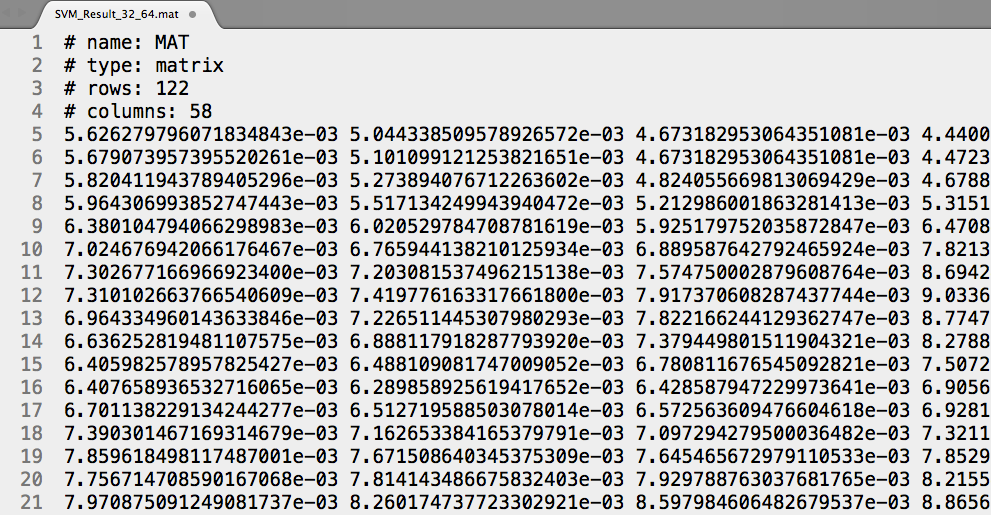
\includegraphics[scale=.4]{images/salida}
  \caption{\em Ejemplo de matriz resultado en el archivo de salida}     
  \label{fig:salida}
\end{figure}
